\documentclass[table]{beamer}
\usepackage[utf8]{inputenc}
\usepackage[brazilian]{babel}
\usepackage{amsmath}
\usepackage{graphicx}
\usepackage{hyperref}
\usepackage{ragged2e}   
\usepackage{epstopdf}
\usepackage{multirow}
\usepackage{minted}
\usepackage{booktabs}

\setbeamertemplate{sidebar right}{}
\setbeamertemplate{footline}{%
\hfill\usebeamertemplate***{navigation symbols}
\hspace{1cm}\insertframenumber{}/\inserttotalframenumber}

\addtobeamertemplate{block begin}{}{\justifying}  %new code

\setbeamertemplate{footline}
{
  \leavevmode%
  \hbox{%
  \begin{beamercolorbox}[wd=.333333\paperwidth,ht=2.25ex,dp=1ex,center]{author in head/foot}%
    \usebeamerfont{author in head/foot}\insertsection
  \end{beamercolorbox}%
  \begin{beamercolorbox}[wd=.333333\paperwidth,ht=2.25ex,dp=1ex,center]{title in head/foot}%
    \usebeamerfont{title in head/foot}\insertsubsection
  \end{beamercolorbox}%
  \begin{beamercolorbox}[wd=.333333\paperwidth,ht=2.25ex,dp=1ex,right]{date in head/foot}%
    \usebeamerfont{date in head/foot}\insertshortdate{}\hspace*{2em}
    \insertframenumber{} / \inserttotalframenumber\hspace*{2ex} 
  \end{beamercolorbox}}%
  \vskip0pt%
}

\begin{document}

\begin{frame}
   \frametitle{Compiladores}
   \large
   \begin{center}
   Ambientes de Execução
   \end{center}
   \scriptsize
   \begin{center}
      João Marcelo Uchôa de Alencar \\
      joao.marcelo@ufc.br \\
      UFC-Quixadá
   \end{center}
\end{frame}

\begin{frame}
   \tableofcontents
\end{frame}

\section{Introdução}
\begin{frame}
   \frametitle{Introdução}
   \begin{itemize}
      \item As análises \textbf{Léxica}, \textbf{Sintática} e \textbf{Semântica} dependem quase que apenas das propriedades da linguagem;
      \item um \textbf{Ambiente de Execução} permite uma representação geral da arquitetura da máquina alvo, como foco nos \textbf{registradores} e \textbf{memória}; 
      \begin{itemize}
         \item estáticos;
	 \item baseados em pilhas;
	 \item dinâmico.
      \end{itemize}
      \item escopo e alocação, ativações de procedimento e passagem de parâmetros;
      \item o papel do compilador é \textbf{indireto}.
   \end{itemize}
\end{frame}

\section{Organização da Memória}
\begin{frame}
   \frametitle{Organização da Memória}
   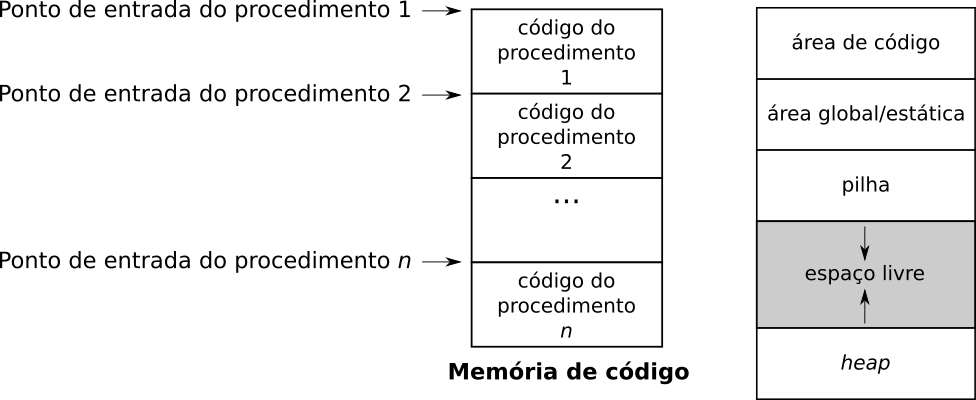
\includegraphics[width=\linewidth,height=\textheight,keepaspectratio]{figuras/organizacaomemoria.png}
\end{frame}

\begin{frame}
   \frametitle{Organização da Memória}
   \begin{itemize}
      \item Área de dados;
      \item área de código;
      \item os endereços e conteúdo da área de código são definidos de maneira estática pelo compilador;
      \item na realidade, a memória não é contínua;
      \item paginação, segmentação, realocação, etc;
      \item mas o \textbf{sistema operacional} oferece a ilusão de uma memória linear;
      \item o compilador trabalha em cima dessa abstração.
   \end{itemize}
\end{frame}

\begin{frame}
   \frametitle{Organização da Memória}
   \begin{itemize}
      \item Variáveis globais podem ter endereço já definido na compilação;
      \item constantes pequenas são, em geral, inseridas diretamente no código pelo compilador, evitando alocação de espaço;
      \item organização típica de memória:
      \begin{itemize}
         \item pilha, LIFO (\textit{last-in, first-out});
	 \item \textit{heap}, acesso aleatório.
      \end{itemize}
      \item pode existir uma \textit{pilha} própria do processador, separada da memória virtual;
      \item nesse caso, a pilha do processo é carregada na pilha da arquitetura na mudança de contexto.
   \end{itemize}
\end{frame}

\begin{frame}
   \frametitle{Organização da Memória}
   \begin{center}
   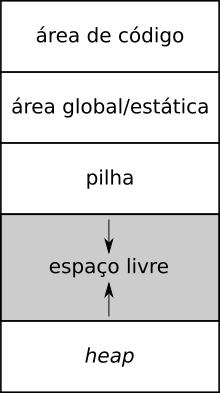
\includegraphics[scale=0.65]{figuras/heappilha.png}
   \end{center}
\end{frame}

\begin{frame}
   \frametitle{Registro de Ativação}
   Contém a memória alocada para os dados locais de um procedimento ou função na medida em que é ativado (ou invocado).
   \begin{center}
   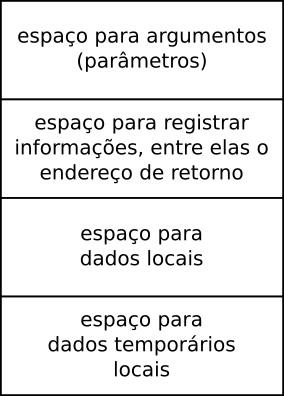
\includegraphics[scale=0.5]{figuras/registroativacao.png}
   \end{center}
\end{frame}

\begin{frame}
   \frametitle{Registro de Ativação}
   \begin{itemize}
      \item Dependendo da linguagem, os registros de ativação podem ser alocados na área estática, na área de pilhas ou área de \textit{heap};
      \item quando forem mantidos na pilha, são denominados \textbf{quadros de pilhas};
      \item os processadores têm registradores para acompanhar a execução: \textbf{contador de programa - pc} e o \textbf{ponteiros de pilhas - sp};
      \item algumas arquiteturas também apresentam o \textbf{ponteiro de quadros - fp} e o \textbf{ponteiro de argumentos - ap};
   \end{itemize}
\end{frame}

\begin{frame}
   \frametitle{Registro de Ativação}
   \begin{block}{Sequência de Ativação}
   Sequência de operações que devem ocorrer quando um procedimento ou função for ativado.
   \end{block}
   \begin{itemize}
      \item Sequência de ativação;
      \item sequência de retorno;
      \item separação das ações entre ativador e ativado:
      \begin{itemize}
         \item o ativador fica responsável pelo tratamento de argumentos;
	 \item salvar o estado da máquina no ponto de ativação.
      \end{itemize}
      \item suporte do processador.
   \end{itemize}
\end{frame}

\section{Ambientes Estáticos}
\begin{frame}
   \frametitle{Ambientes Estáticos}
   \begin{itemize}
      \item Pode ser usado para implementar uma linguagem em que não há ponteiros ou alocação dinâmica, sem procedimentos recursivos;
      \item todas as variáveis são alocadas estaticamente;
      \item todas as variáveis podem ser acessadas diretamente pelos endereços fixos;
      \item cada procedimento tem um único registro de ativação.
   \end{itemize}
\end{frame}

\begin{frame}
   \frametitle{Ambientes Estáticos}
   \begin{center}
      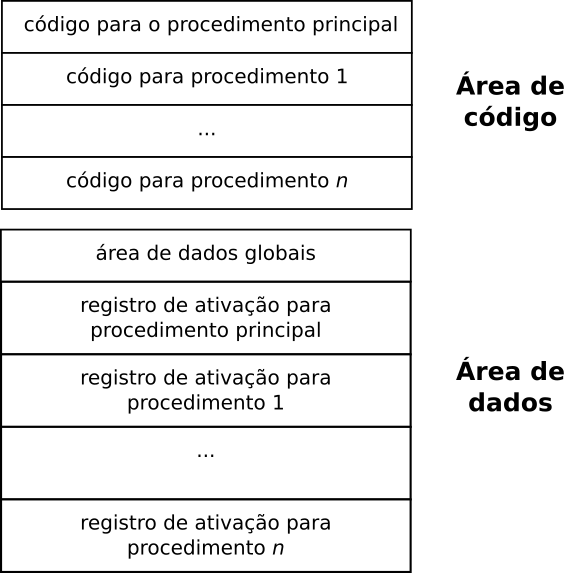
\includegraphics[scale=0.4]{figuras/ambienteestatico.png}
   \end{center}
\end{frame}

\begin{frame}[fragile]
   \frametitle{Ambientes Estáticos}
   \scriptsize
   \begin{minted}{fortran}
   PROGRAM TEST
   COMMON MAXSIZE
   INTEGER MAXSIZE
   REAL TABLE(10), TEMP
   MAXSIZE = 10
   READ *, TABLE(1), TABLE(2), TABLE(3)
   CALL QUADMEAN(TABLE, 3, TEMP)
   PRINT *, TEMP
   END
   
   SUBROUTINE QUADMEAN(A, SIZE, QMEAN)
   COMMON MAXSIZE
   INTEGER MAXSIZE, SIZE
   REAL A(SIZE), QMEAN, TEMP
   INTEGER K
   TEMP = 0.0
   IF ((SIZE.GT.MAXSIZE) .OR. (SIZE.LT.1)) GOTO 99
   DO 10 K = 1, SIZE
      TEMP = TEMP + A(K) * A(K)
10 CONTINUE
99 QMEAN = SQRT(TEMP/SIZE)
   RETURN
   END
   \end{minted}
\end{frame}

\begin{frame}
   \frametitle{Ambientes Estáticos}
   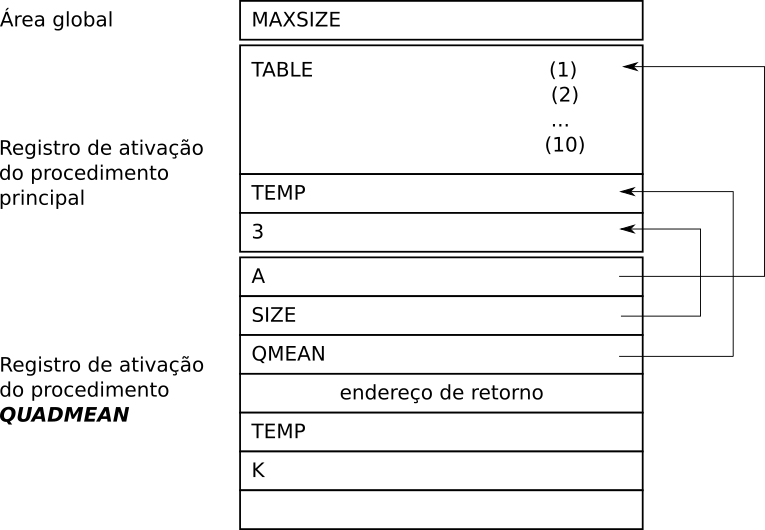
\includegraphics[width=\linewidth,height=\textheight,keepaspectratio]{figuras/ambienteestaticoativacao.png}
\end{frame}

\section{Ambientes em Pilhas}
\begin{frame}
   \frametitle{Ambientes de Execução Baseado em Pilhas}
   Ambientes em Pilhas são necessários para linguagens que permitam \textbf{ativações recursivas} e \textbf{variáveis locais} com novas alocações a cada ativação.
   \begin{itemize}
      \item Uma \textbf{pilha de registros de ativação} é usada para armazenar os registros de ativação;
      \item cada função ou procedimento pode ter vários registros distintos na pilha ao mesmo tempo, cada um representando uma invocação distinta;
      \item é necessário que o compilador construa uma tabela de símbolos capaz de referenciar as variáveis corretas de acordo com o caminho da execução.
   \end{itemize}
\end{frame}

\begin{frame}
   \frametitle{Ambientes em Pilhas sem Procedimentos Locais}
   Em linguagens como C, todos os procedimentos (funções) são globais. O ambiente precisa garantir duas coisas:
   \begin{enumerate}
      \item Um ponteiro que aponte para o registro de ativação corrente, para permitir o acesso a variáveis locais;
      \item armazenar a posição ou tamanho do registro de ativação anterior, para permitir o retorno quando a invocação corrente for finalizada.
   \end{enumerate}
   Para atender esses requisitos, temos então:
   \begin{itemize}
      \item \textbf{Ponteiro de quadro} ou \textbf{fp} (\textit{frame pointer}), armazenado em um registrador;
      \item Um campo de \textbf{vinculação de controle} ou \textbf{vinculação dinâmica} na ativação corrente, que contém o valor anterior de \textbf{fp}.
   \end{itemize}
   O topo da pilha é armazenado no \textbf{ponteiro de pilha} ou \textbf{sp} (\textit{stack pointer}).
\end{frame}

\begin{frame}[fragile]
   \frametitle{Ambientes em Pilhas sem Procedimentos Locais}
   \begin{minted}{c}
#include <stdio.h>

int x, y;

int gcd(int u, int v) {
   if (v == 0) return u;
   else return gcd(v, u % v);
}

int main(int argc, char *argv[]) {
  scanf("%d%d", &x, &y);
  printf("%d\n", gcd(x, y));
  return 0;
}
   \end{minted}
   Vamos considerar a execução do programa com os valores $(15,10)$.
\end{frame}

\begin{frame}
   \frametitle{Ambientes em Pilhas sem Procedimentos Locais}
   \begin{center}
   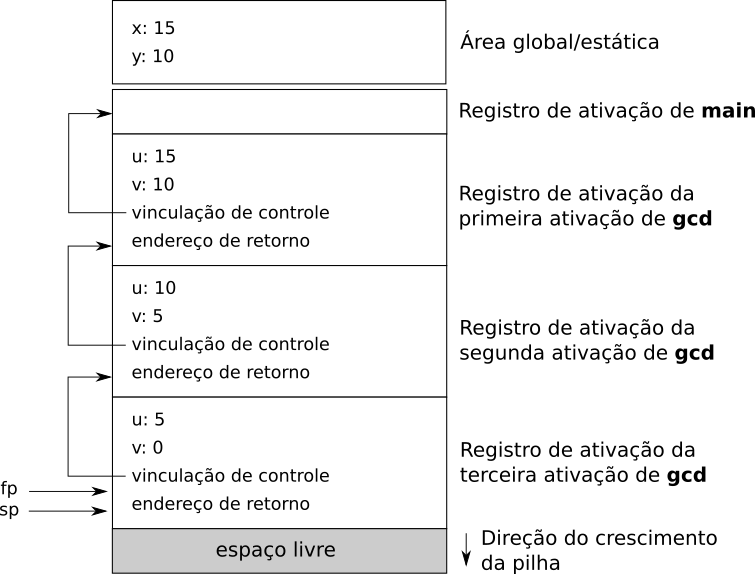
\includegraphics[scale=0.4]{figuras/ambientebaseadoempilhas01.png}
   \end{center}
\end{frame}

\begin{frame}[fragile]
   \frametitle{Ambientes em Pilhas sem Procedimentos Locais}
   \begin{columns}
   \begin{column}{0.4\textwidth}
   \scriptsize
   \begin{minted}{c}
int x = 2;
void g(int); /* protótipo */

void f(int n) {
  static int x = 1;
  g(n);
  x--;
}

void g(int m) {
  int y = m - 1;
  if (y > 0) {
     f(y);
     x--;
     g(y);
  }
}

main() {
   g(x);
   return 0;
}
   \end{minted}
   \end{column}
   \begin{column}{0.6\textwidth}
   \scriptsize
   \begin{enumerate}
      \item A primeira ativação em $main$ é $g(2)$ ($m=2$, $y=1$);
      \item $g$ ativa $f(1)$ ($n=1$) e $f$ ativa $g(1)$ ($m=1$, $y=0$);
      \item a partir daí não há mais ativações. 
   \end{enumerate}
   \vspace{0.5cm}
   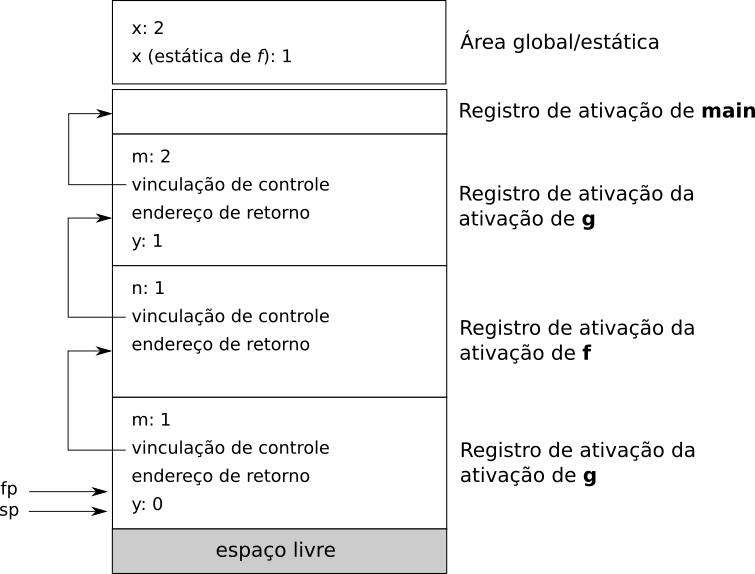
\includegraphics[scale=0.3]{figuras/ambientebaseadoempilhas02.png}
   \end{column}
   \end{columns}
\end{frame}

\begin{frame}[fragile]
   \frametitle{Ambientes em Pilhas sem Procedimentos Locais}
   \begin{columns}
   \begin{column}{0.4\textwidth}
   \scriptsize
   \begin{enumerate}
      \item As ativações de $g$ e $f$ são encerradas;
      \item os registros de ativação são retirados e o controle é devolvido para $g$;
      \item $x$ é decrementado;
      \item $g(1)$ é ativado ($m=1$, $y=0$).
   \end{enumerate}
   \end{column}
   \begin{column}{0.6\textwidth}
   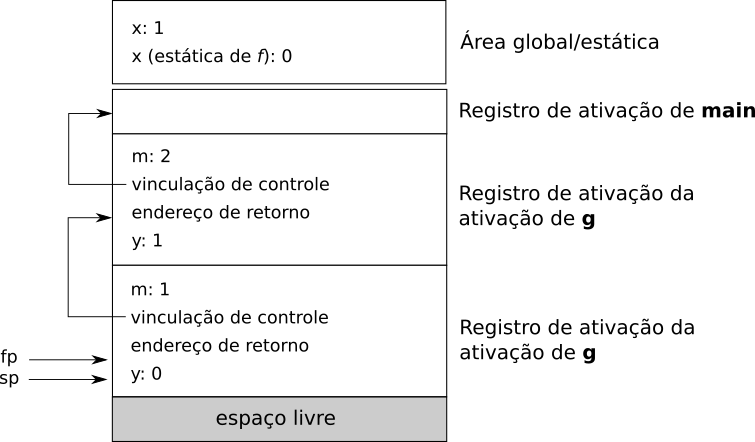
\includegraphics[scale=0.3]{figuras/ambientebaseadoempilhas03.png}
   \end{column}
   \end{columns}
   \vspace{1.0cm}
   Não ocorre confusão com a variável externa $x$, pois a tabela de símbolos as diferencia.
\end{frame}

\begin{frame}[fragile]
   \frametitle{Ambientes em Pilhas sem Procedimentos Locais}
   \begin{block}{Acesso a nomes}
   O compilador deve calcular o deslocamento para acessar as variáveis locais e parâmetros a partir da base do registro de ativação ou quadro corrente, armazenando esse valor na tabela.
   \end{block}
   Considerando a função $g$ do exemplo anterior:
   \begin{center}
   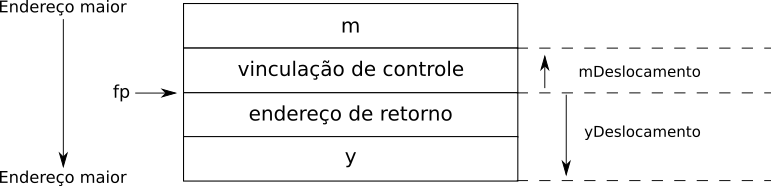
\includegraphics[scale=0.4]{figuras/ambientebaseadoempilhas04.png}
   \end{center}
   Com endereços de 4 \textit{bytes} e inteiros de 2 \textit{bytes}:
   \begin{minted}{pascal}
   mDeslocamento = +4, 4(fp)
   yDeslocamento = -6, -6(fp)
   \end{minted}
\end{frame}

\begin{frame}[fragile]
   \frametitle{Ambientes em Pilhas sem Procedimentos Locais}
   \begin{minted}{c}
void f(int x, char c) {
   int a[10];
   double y;
   ...
}
   \end{minted}
   \begin{center}
   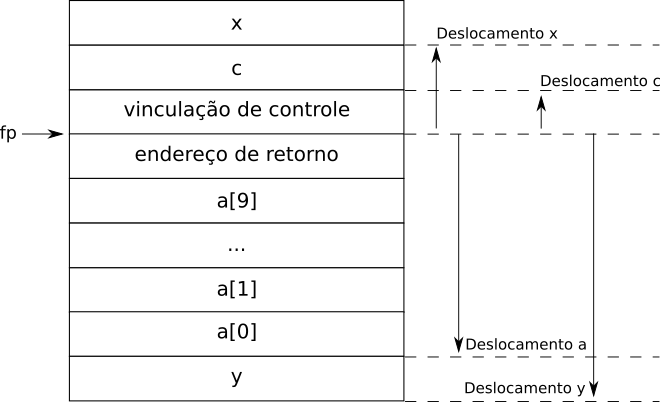
\includegraphics[scale=0.4]{figuras/ambientebaseadoempilhas05.png}
   \end{center}
\end{frame}

\begin{frame}
   \frametitle{Ambientes em Pilhas sem Procedimentos Locais}
   \begin{table}
   \begin{tabular}{l|c}
   Nome & Deslocamento \\
   \hline
   x & +5 \\
   c & +4 \\
   a & -24 \\
   y & -32 \\
   \hline 
   \end{tabular}
   \\
   \vspace{1.0cm}
   Um acesso a $a[i]$ requer que o compilador defina uma função para calcular o endereço $(-24 + 2 * i) (fp)$. Variáveis globais e estáticas tem seu endereço definido de forma estática pelo compilador, em função do endereço inicial do programa.
\end{table}
\end{frame}

\begin{frame}
   \frametitle{Sequência de Ativação}
   \begin{enumerate}
      \item Compute os argumentos e os armazene nas posições corretas no novo registro de ativação do procedimento (colocá-los na pilha de execução em ordem produzirá esse efeito);
      \item armazene (coloque na pilha) o $fp$ e a vinculação de controle no novo registro de ativação;
      \item modifique o $fp$ para que ele aponte para o começo do novo registro de ativação (se houver um $sp$, a cópia do $sp$ no $fp$ nesse ponto produzirá esse efeito);
      \item armazene o endereço de retorno no novo registro de ativação;
      \item efetue um salto para o código do procedimento ativado.
   \end{enumerate}
\end{frame}

\begin{frame}
   \frametitle{Encerramento de Procedimento}
   \begin{enumerate}
      \item Copie o $fp$ no $sp$;
      \item carregue a vinculação de controle no $fp$;
      \item efetue um salto para o endereço de retorno;
      \item altere $sp$ para retirar da pilha de argumentos.
   \end{enumerate}
\end{frame}

\begin{frame}
   \frametitle{Exemplo de Sequência de Ativação}
   Considere a situação anterior a última ativação de $g$ no exemplo. \\
   \begin{center}
   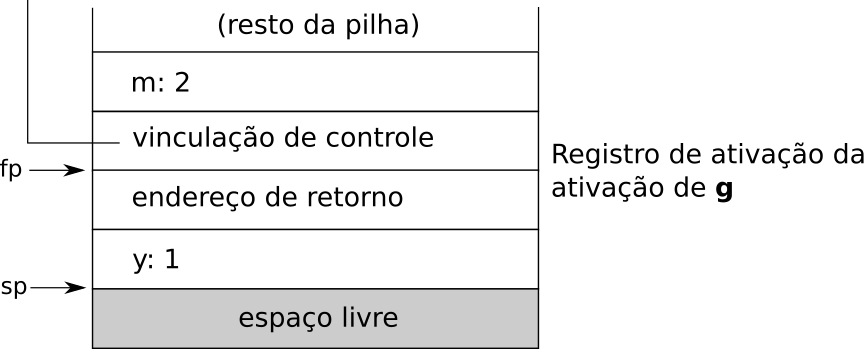
\includegraphics[width=\linewidth,height=\textheight,keepaspectratio]{figuras/sequenciaativacao01.png}
   \end{center}
\end{frame}

\begin{frame}
   \frametitle{Exemplo de Sequência de Ativação}
   Quando a nova ativação de $g$ for efetuada, primeiro o valor do parâmetro de $m$ será colocado na pilha de execução: \\
   \begin{center}
   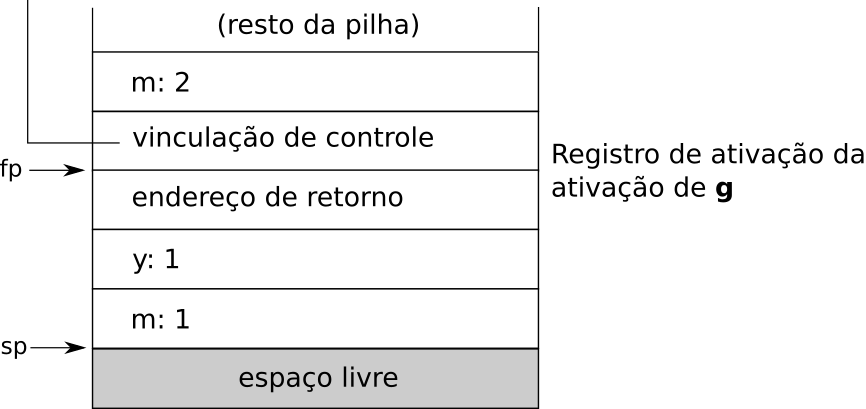
\includegraphics[width=\linewidth,height=\textheight,keepaspectratio]{figuras/sequenciaativacao02.png}
   \end{center}
\end{frame}

\begin{frame}
   \frametitle{Exemplo de Sequência de Ativação}
   O $fp$ é, em seguida, colocado na pilha: \\
   \begin{center}
   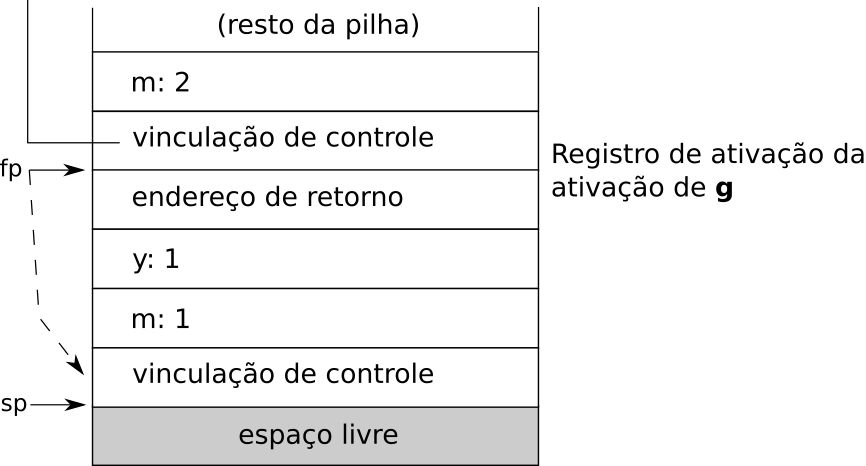
\includegraphics[width=\linewidth,height=\textheight,keepaspectratio]{figuras/sequenciaativacao03.png}
   \end{center}
\end{frame}

\begin{frame}
   \frametitle{Exemplo de Sequência de Ativação}
   $sp$ é copiado no $fp$, o endereço de retorno é colocado na pilha e é efetuado o salto para a nova ativação de $g$: \\
   \begin{center}
   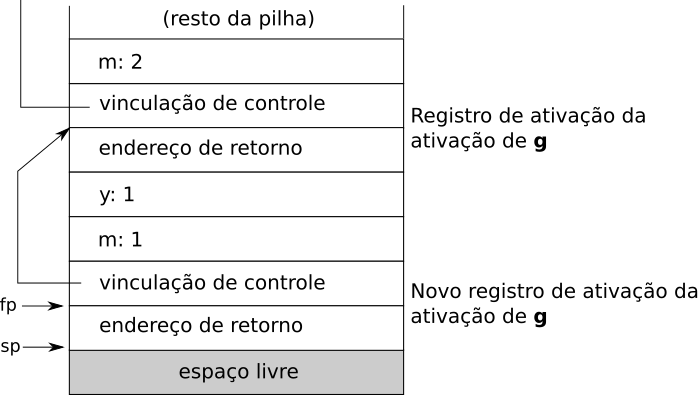
\includegraphics[width=\linewidth,height=\textheight,keepaspectratio]{figuras/sequenciaativacao04.png}
   \end{center}
\end{frame}

\begin{frame}
   \frametitle{Exemplo de Sequência de Ativação}
   $g$ aloca e fornece o valor inicial ao novo $y$ na pilha: \\
   \begin{center}
   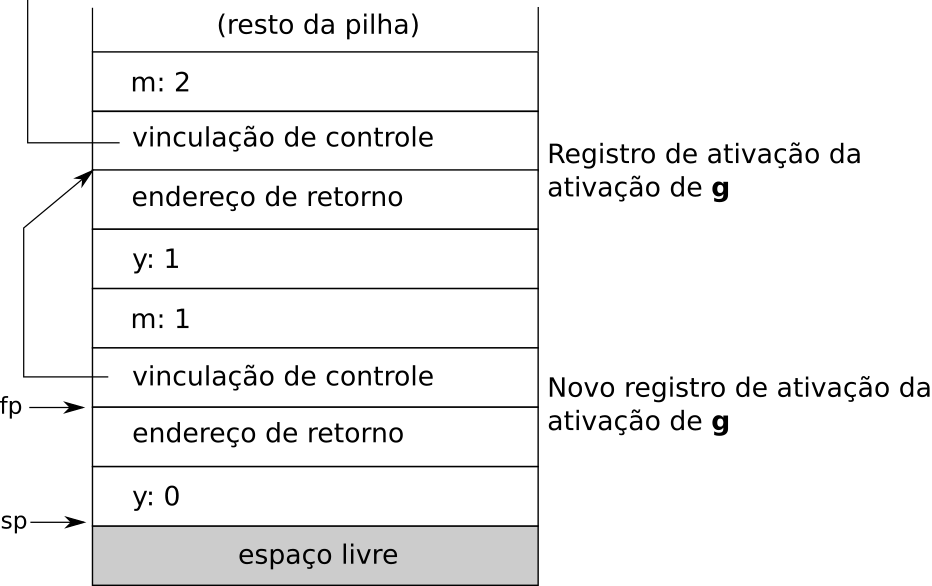
\includegraphics[width=\linewidth,height=\textheight,keepaspectratio]{figuras/sequenciaativacao05.png}
   \end{center}
\end{frame}

\begin{frame}[fragile]
   \frametitle{Dados de Comprimento Variável}
   O que fazer quando:
   \begin{itemize}
      \item A quantidade de argumentos em uma ativação pode variar de uma ativação para outra?
      \item o tamanho de um parâmetro de tipo matriz ou de uma variável de tipo matriz pode variar de uma ativação para outra.
   \end{itemize}
   Um exemplo é a função \textsf{printf} em C:
   \begin{minted}{c}
   // Quatro argumentos
   printf("%d%s%c", n, prompt, ch);
   // Um argumento
   print("Olá, Mundo\n");
   \end{minted}
   Os compiladores em C tratam essa situação percorrendo toda a lista de parâmetros e colocando os argumentos no registro de ativação na \textbf{ordem inversa}.
\end{frame}

\begin{frame}[fragile]
   \frametitle{Temporários Locais e Declarações Aninhadas}
   Considere a expressão em C:
   \begin{minted}{c}
   x[i] = (i+j)*(i/k+f(j))
   \end{minted}
   Três resultados parciais são gravados antes da ativação de $f$:
   \begin{enumerate}
      \item $x[i]$;
      \item $i+j$;
      \item $i/k$.
   \end{enumerate}
   Esses dados são armazenados temporariamente na pilha de execução, entre o registro de ativação e o novo registro criado a partir da invocação de $f$.
\end{frame}

\begin{frame}[fragile]
   \frametitle{Ambientes em Pilhas com Procedimentos Locais}
   \footnotesize
   \begin{minted}{pascal}
program nonLocalRef;
procedure p;
var n:integer;
   procedure q;
   begin
      (* uma referência a n é 
         agora não local e não global *)
   end; (* q *)
   procedure r(n: integer);
   begin
      q;
   end; (* r *)
begin (* p *)
   n := 1;
   r(2);
end; (* p *)
begin (* main *)
   p;
end.
   \end{minted}
\end{frame}

\begin{frame}
   \frametitle{Ambientes em Pilhas com Procedimentos Locais}
   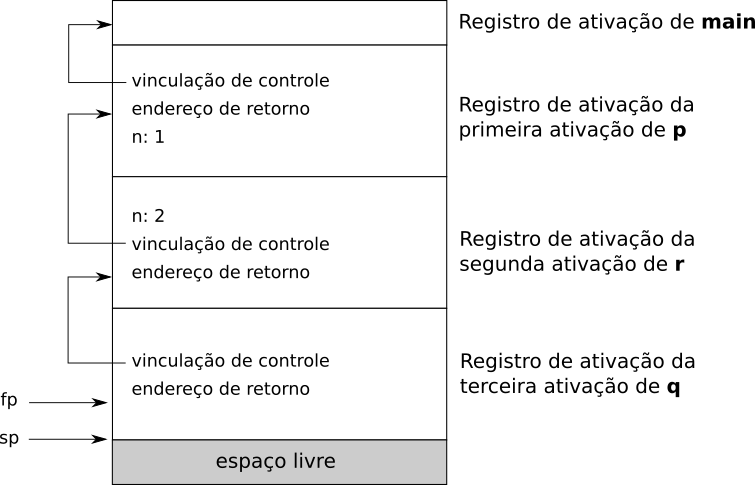
\includegraphics[width=\linewidth,height=\textheight,keepaspectratio]{figuras/procedimentoslocais01.png}
\end{frame}

\begin{frame}
   \frametitle{Ambientes em Pilhas com Procedimentos Locais}
   \begin{itemize}
      \item De acordo com o escopo estático, referências a $n$ em $q$ devem apontar a variável local $n$ de $p$;
      \item não é possível encontrá-la através das vinculações de controle;
      \item o escopo dinâmico resolve o problema, mas é o que desejamos;
      \item a solução é adicionar mais um campo no registro, a \textbf{vinculação de acesso}.
   \end{itemize}
\end{frame}

\begin{frame}
   \frametitle{Ambientes em Pilhas com Procedimentos Locais}
   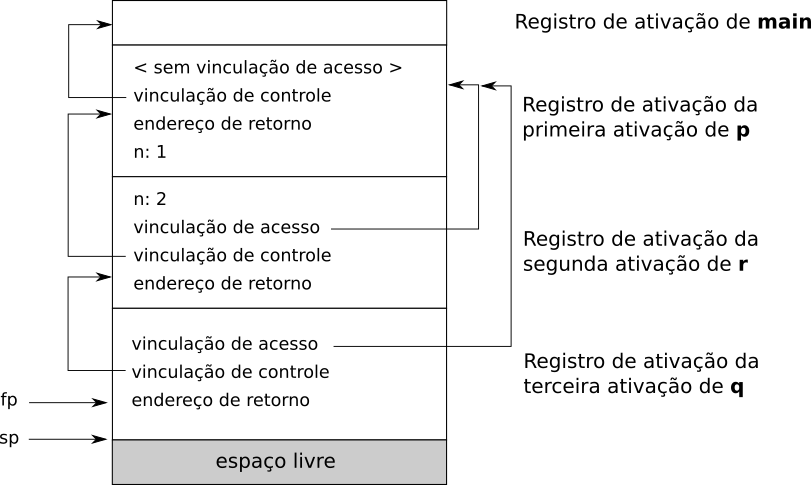
\includegraphics[width=\linewidth,height=\textheight,keepaspectratio]{figuras/procedimentoslocais02.png}
\end{frame}

\begin{frame}[fragile]
   \frametitle{Ambientes em Pilhas com Procedimentos Locais}
   \small
   \begin{minted}{pascal}
program chain;
procedure p;
var x: integer;
   procedure q;
      procedure r;
      begin
         x := 2;
	 ...
	 if ... then p;
      end; (* r *)
   begin
      r;
   end; (* q *)
begin
   q;
end; (* p *)
begin (* main *)
   p;
end.
   \end{minted}
\end{frame}

\begin{frame}
   \frametitle{Ambientes em Pilhas com Procedimentos Locais}
   \begin{itemize}
      \item O compilador define o nível de escopo de cada declaração e procedimento;
      \item já vimos como isso pode ser feito através de atributos na análise semântica;
      \item \textbf{nível de aninhamento};
      \item \textbf{encadeamento de acesso}.
   \end{itemize}
\end{frame}

\begin{frame}
   \frametitle{Ambientes em Pilhas com Parâmetros de Procedimentos}
   \begin{itemize}
      \item Em algumas linguagens, procedimentos podem ser passados como parâmetros;
      \item a vinculação de acesso deve ser pré-computada e passada junto com um ponteiro para o código;
      \item \textbf{fechamento:}
      \begin{itemize}
         \item ponteiro de instrução;
	 \item ponteiro de ambiente.
      \end{itemize}
      \item $<ip, ep>$.
   \end{itemize}
\end{frame}

\begin{frame}[fragile]
   \frametitle{Ambientes em Pilhas com Procedimentos Locais}
   \small
   \begin{minted}{pascal}
program closureEx(output);
procedure p(procedure a);
begin
   a;
end;
procedure q;
var x:integer;
   procedure r;
   begin
      writeln(x);
   end;
begin
   x := 2;
   p(r);
end; (* q *)

begin (* main *)
   q;
end.
   \end{minted}
\end{frame}

\begin{frame}
   \frametitle{Ambientes em Pilhas com Procedimentos Locais}
   \begin{columns}
   \begin{column}{0.5\textwidth}
   Logo após ativação de $p$.
   \begin{center}
   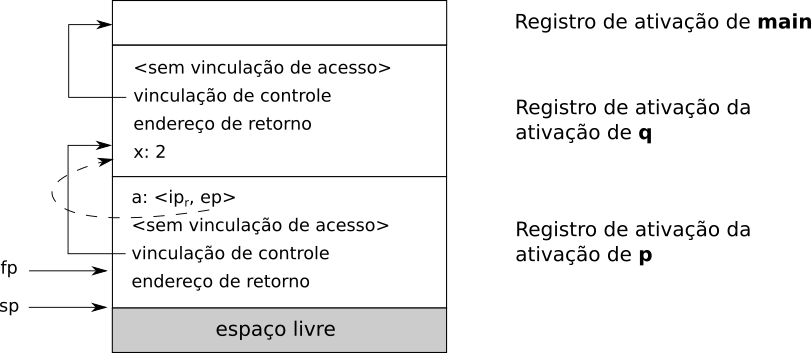
\includegraphics[width=\linewidth,height=\textheight,keepaspectratio]{figuras/procedimentosparametros01.png}
   \end{center}
   \end{column}
   \begin{column}{0.5\textwidth}
   Após ativação de  $a$.
   \begin{center}
   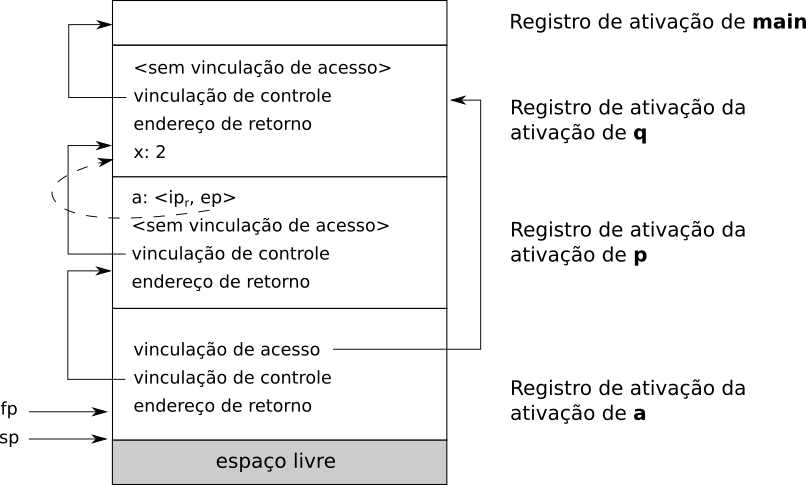
\includegraphics[width=\linewidth,height=\textheight,keepaspectratio]{figuras/procedimentosparametros02.png}
   \end{center}
   \end{column}
   \end{columns}
\end{frame}

\section{Memória Dinâmica}
\begin{frame}[fragile]
   \frametitle{Memória Dinâmica}
   \begin{itemize}
      \item A gerência da pilha até agora não é suficiente para linguagens nas quais uma referência auma variável local pode ser retornada ao ativador:
      \begin{minted}{c}
// Referência pendente
int *dangle(void) {
   int x;
   return &x;
}
      \end{minted}
      \item outro problema é quando a linguagem permite procedimentos locais que também podem ser retornados;
      \item a solução é manter os registros de ativação até que são sejam mais referenciados;
      \item \textbf{coleta de lixo}.
\end{itemize}
\end{frame}

\begin{frame}
   \frametitle{Memória Dinâmica em Linguagens Orientadas a Objetos}
   \begin{itemize}
      \item Um objeto na memória é um cruzamento entre uma estrutura de registros e um registro de ativação;
      \item a solução mais simples é fazer cada objeto copiar todos os atributos e métodos herdados para sua memória;
      \item um alternativa é manter toda a estrutura de classes na memória através de um \textbf{grafo de heranças};
      \item uma solução intermediária é definir uma \textbf{tabela de função virtual}.
   \end{itemize}
\end{frame}

\begin{frame}
   \frametitle{Gerência de \textit{Heap}}
   \begin{itemize}
      \item Duas operações: \textit{alocar} e \textit{liberar};
      \item \textit{alocar} recebe um tamanho em \textit{bytes} e reserva blocos de memória, retornando o primeiro endereço do bloco;
      \item \textit{liberar} recebe o endereço inicial e marca um bloco como livre;
      \item pode ser implementada como uma lista de encadeadas de blocos livres, o que pode levar fragmentação;
      \item uma solução melhor é uma lista encadeada circular para os blocos alocados e livres.
   \end{itemize}
\end{frame}

\begin{frame}
   \frametitle{Gerência Automática de \textit{Heap}}
   \begin{itemize}
      \item \textbf{Coleta de Lixo}: recuperação do espaço previamente alocado mas não mais em um uso, sem uma ativação explícita de \textit{liberar};
      \item \textbf{marcar e varrer};
      \item \textbf{parar e copiar};
      \item \textbf{coleta de lixo gerativa}.
   \end{itemize}
\end{frame}

\section{Passagem de Parâmetros}
\begin{frame}
   \frametitle{Passagem de Parâmetros}
   \begin{itemize}
      \item Passagem por valor;
      \item passagem por referência;
      \item passagem por valor-resultado;
      \item passagem por nome.
   \end{itemize}
\end{frame}

\begin{frame}
   \frametitle{Conclusão}
   Dúvidas?
\end{frame}

\end{document}
